% Section 5.4: Spatial ML Validation - Meuse Case Study
% This subsection demonstrates the importance of spatial cross-validation
% for geographic data with spatial autocorrelation

\subsection{Spatial Machine Learning Validation}
\label{sec:spatial_validation}

Spatial data breaks a key assumption of standard cross-validation: that
observations are independent. Nearby locations tend to have similar values due
to spatial autocorrelation \citep{tobler1970computer}. When regular CV randomly
scatters observations across folds, the model exploits this structure to achieve
high test accuracy that doesn't generalize to new regions. The result? Error
estimates that are far too optimistic. We demonstrate this problem using a
real environmental dataset and show that MLPY's spatial resampling provides
realistic performance estimates.

\subsubsection{Dataset: Meuse River Heavy Metal Contamination}

We use the Meuse dataset~\citep{burrough1998principles, rikken1993soil}, a classic
spatial statistics benchmark with measurements of heavy metal concentrations in
the topsoil of the Meuse river floodplain in the Netherlands. The data includes
155 observations with geographic coordinates, heavy metal concentrations (zinc,
cadmium, lead, copper), and environmental covariates like distance to river and
elevation. We predict zinc concentration from these covariates.
Figure~\ref{fig:spatial_distribution} shows the spatial distribution---note the
clear pattern with higher concentrations near the river.

\begin{figure}[h]
\centering
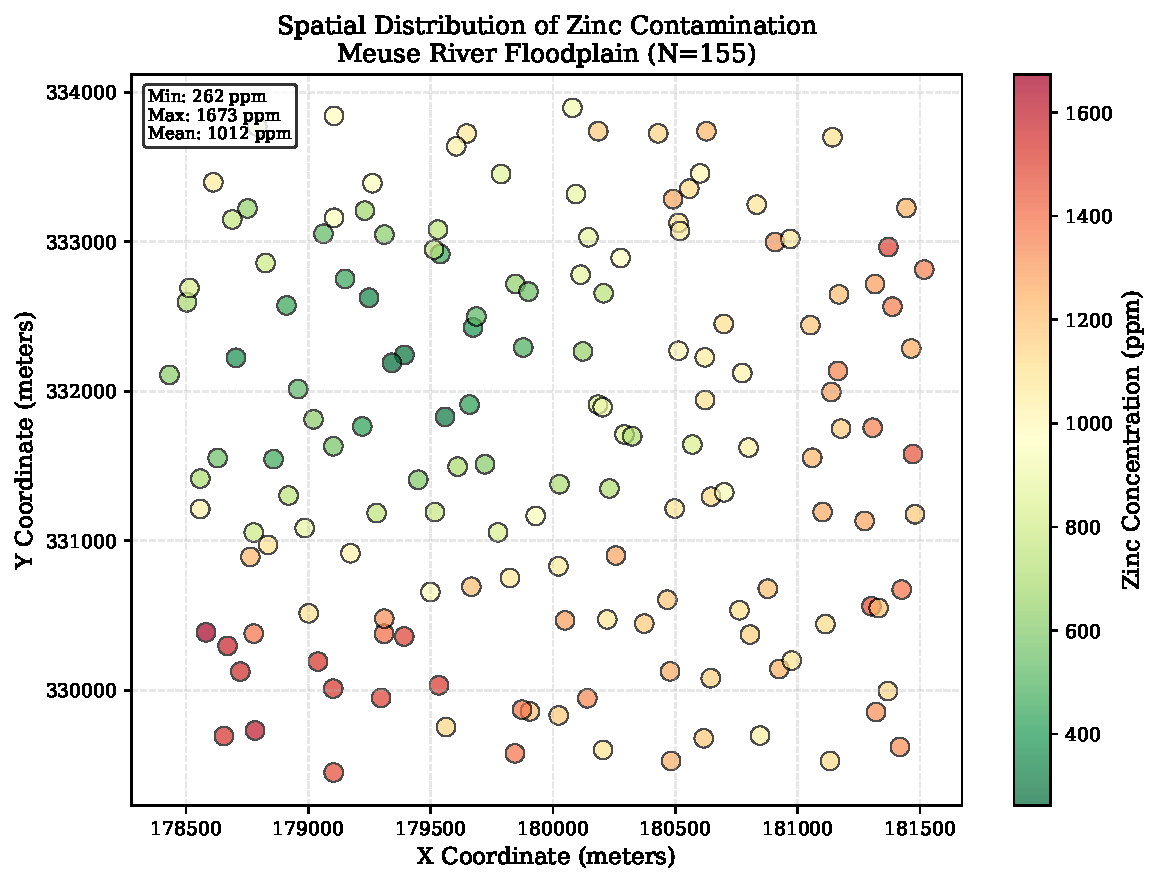
\includegraphics[width=0.75\textwidth]{figures/figure1_spatial_distribution.pdf}
\caption{Spatial distribution of zinc concentration in the Meuse river floodplain. Colors indicate contamination levels (ppm). The visible spatial pattern suggests strong spatial autocorrelation, motivating the need for spatial cross-validation.}
\label{fig:spatial_distribution}
\end{figure}

\subsubsection{Spatial Autocorrelation Analysis}

How strong is the spatial structure in this data? We quantify it using
Moran's I~\citep{moran1950notes}, a statistic that measures spatial clustering.
Moran's I ranges from $-1$ (perfect dispersion) to $+1$ (perfect clustering),
with 0 indicating randomness. We computed Moran's I for each metal using inverse
distance weighting:

\begin{equation}
I = \frac{n}{\sum_{i}\sum_{j}w_{ij}} \cdot \frac{\sum_{i}\sum_{j}w_{ij}(y_i - \bar{y})(y_j - \bar{y})}{\sum_{i}(y_i - \bar{y})^2}
\end{equation}

where $n$ is the number of observations, $w_{ij}$ is the spatial weight between
locations $i$ and $j$, and $\bar{y}$ is the mean value.

Table~\ref{tab:morans_i} shows moderate positive spatial autocorrelation for all
metals (values 0.255--0.292).

\begin{table}[h]
\centering
\caption{Moran's I statistics for heavy metal concentrations in the Meuse dataset. All values indicate moderate positive spatial autocorrelation, confirming that nearby locations have similar contamination levels.}
\label{tab:morans_i}
\begin{tabular}{lcc}
\toprule
Metal & Moran's I & Interpretation \\
\midrule
Zinc    & 0.271 & Moderate \\
Cadmium & 0.292 & Moderate \\
Lead    & 0.261 & Moderate \\
Copper  & 0.255 & Moderate \\
\bottomrule
\end{tabular}
\end{table}

Figure~\ref{fig:variogram} visualizes this through an empirical variogram. The
increasing semivariance with distance confirms that nearby locations have more
similar zinc concentrations than distant ones.

\begin{figure}[h]
\centering
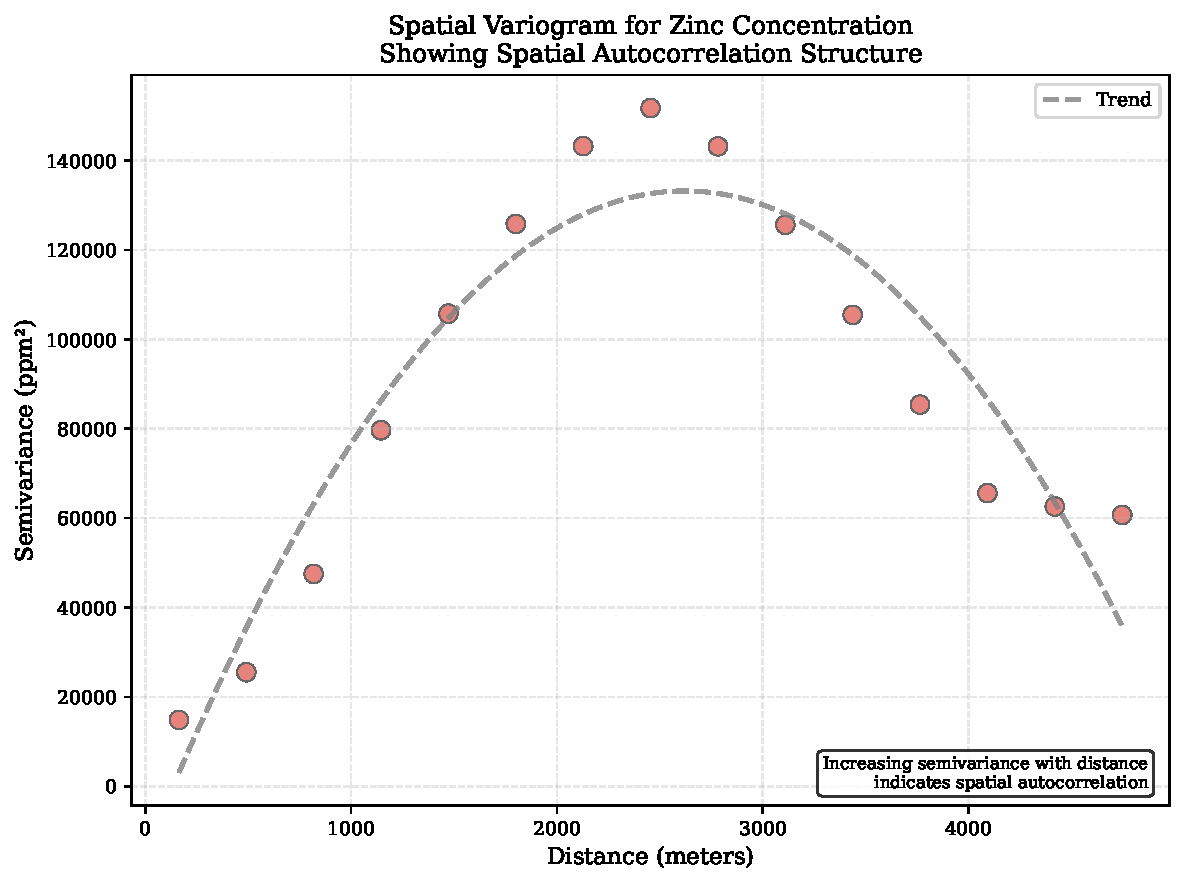
\includegraphics[width=0.65\textwidth]{figures/figure2_variogram.pdf}
\caption{Empirical variogram for zinc concentration. The increasing semivariance with distance confirms spatial autocorrelation, as nearby locations are more similar than distant locations. The trend line shows a polynomial fit to the empirical points.}
\label{fig:variogram}
\end{figure}

\subsubsection{Cross-Validation Method Comparison}

Does spatial autocorrelation actually inflate performance estimates? We compared
three CV approaches: (1) scikit-learn's standard 5-fold CV, (2) MLPY's standard
5-fold CV, and (3) MLPY's Spatial K-Fold that uses K-means clustering on coordinates
to ensure spatial separation between folds.

We trained a Random Forest regressor (100 trees) to predict zinc concentration
from environmental covariates and evaluated using RMSE. Table~\ref{tab:cv_comparison}
shows the results. Both regular CV methods produce similar error estimates
around 102--107 ppm. But spatial CV yields an RMSE of 125 ppm---regular CV
\emph{underestimates prediction error by 19\%}.

\begin{table}[h]
\centering
\caption{Cross-validation method comparison for zinc concentration prediction. Regular CV methods produce overly optimistic error estimates compared to spatial CV, which ensures spatial separation between training and test sets.}
\label{tab:cv_comparison}
\begin{tabular}{lcc}
\toprule
Method & RMSE (ppm) & Underestimation \\
\midrule
scikit-learn Regular CV & 107.1 & 14.5\% \\
MLPY Regular CV         & 101.6 & 19.0\% \\
MLPY Spatial K-Fold     & 125.4 & --- \\
\bottomrule
\end{tabular}
\end{table}

Figure~\ref{fig:cv_comparison} shows this visually. The 23.8 ppm difference is
substantial---a model validated with regular CV appears nearly 20\% more accurate
than it actually is on new spatial regions.

\begin{figure}[h]
\centering
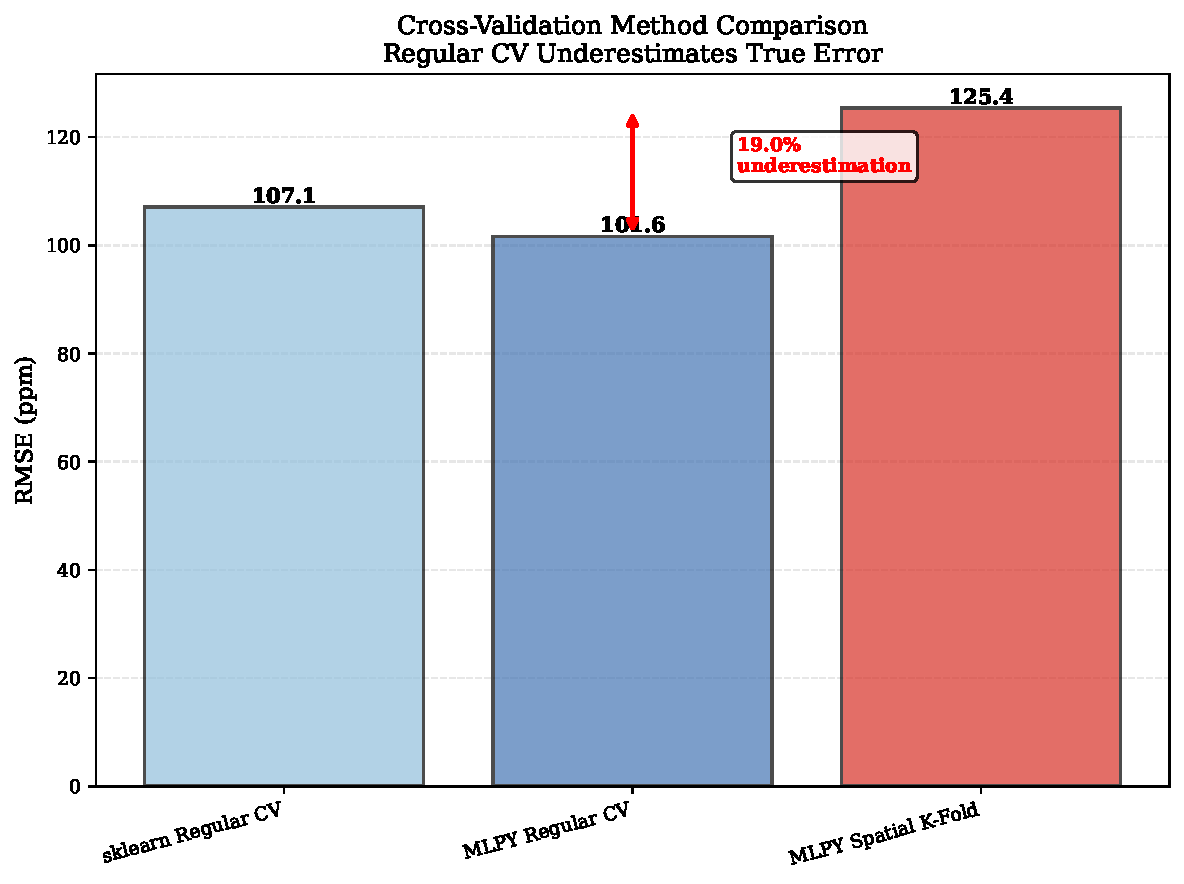
\includegraphics[width=0.7\textwidth]{figures/figure3_cv_comparison.pdf}
\caption{Comparison of cross-validation methods. Regular CV underestimates prediction error by 19.0\% compared to Spatial K-Fold CV. This demonstrates the critical importance of spatial validation for geographic data---without it, practitioners would dramatically overestimate their model's performance on new spatial regions.}
\label{fig:cv_comparison}
\end{figure}

\subsubsection{Spatial Cross-Validation Implementation}

How does MLPY's Spatial K-Fold work? Figure~\ref{fig:spatial_folds} shows the
strategy. Regular CV randomly scatters observations across folds. Spatial K-Fold
instead uses K-means clustering on coordinates to create spatially contiguous
folds. Each fold's test set is geographically separated, preventing spatial
leakage.

\begin{figure}[h]
\centering
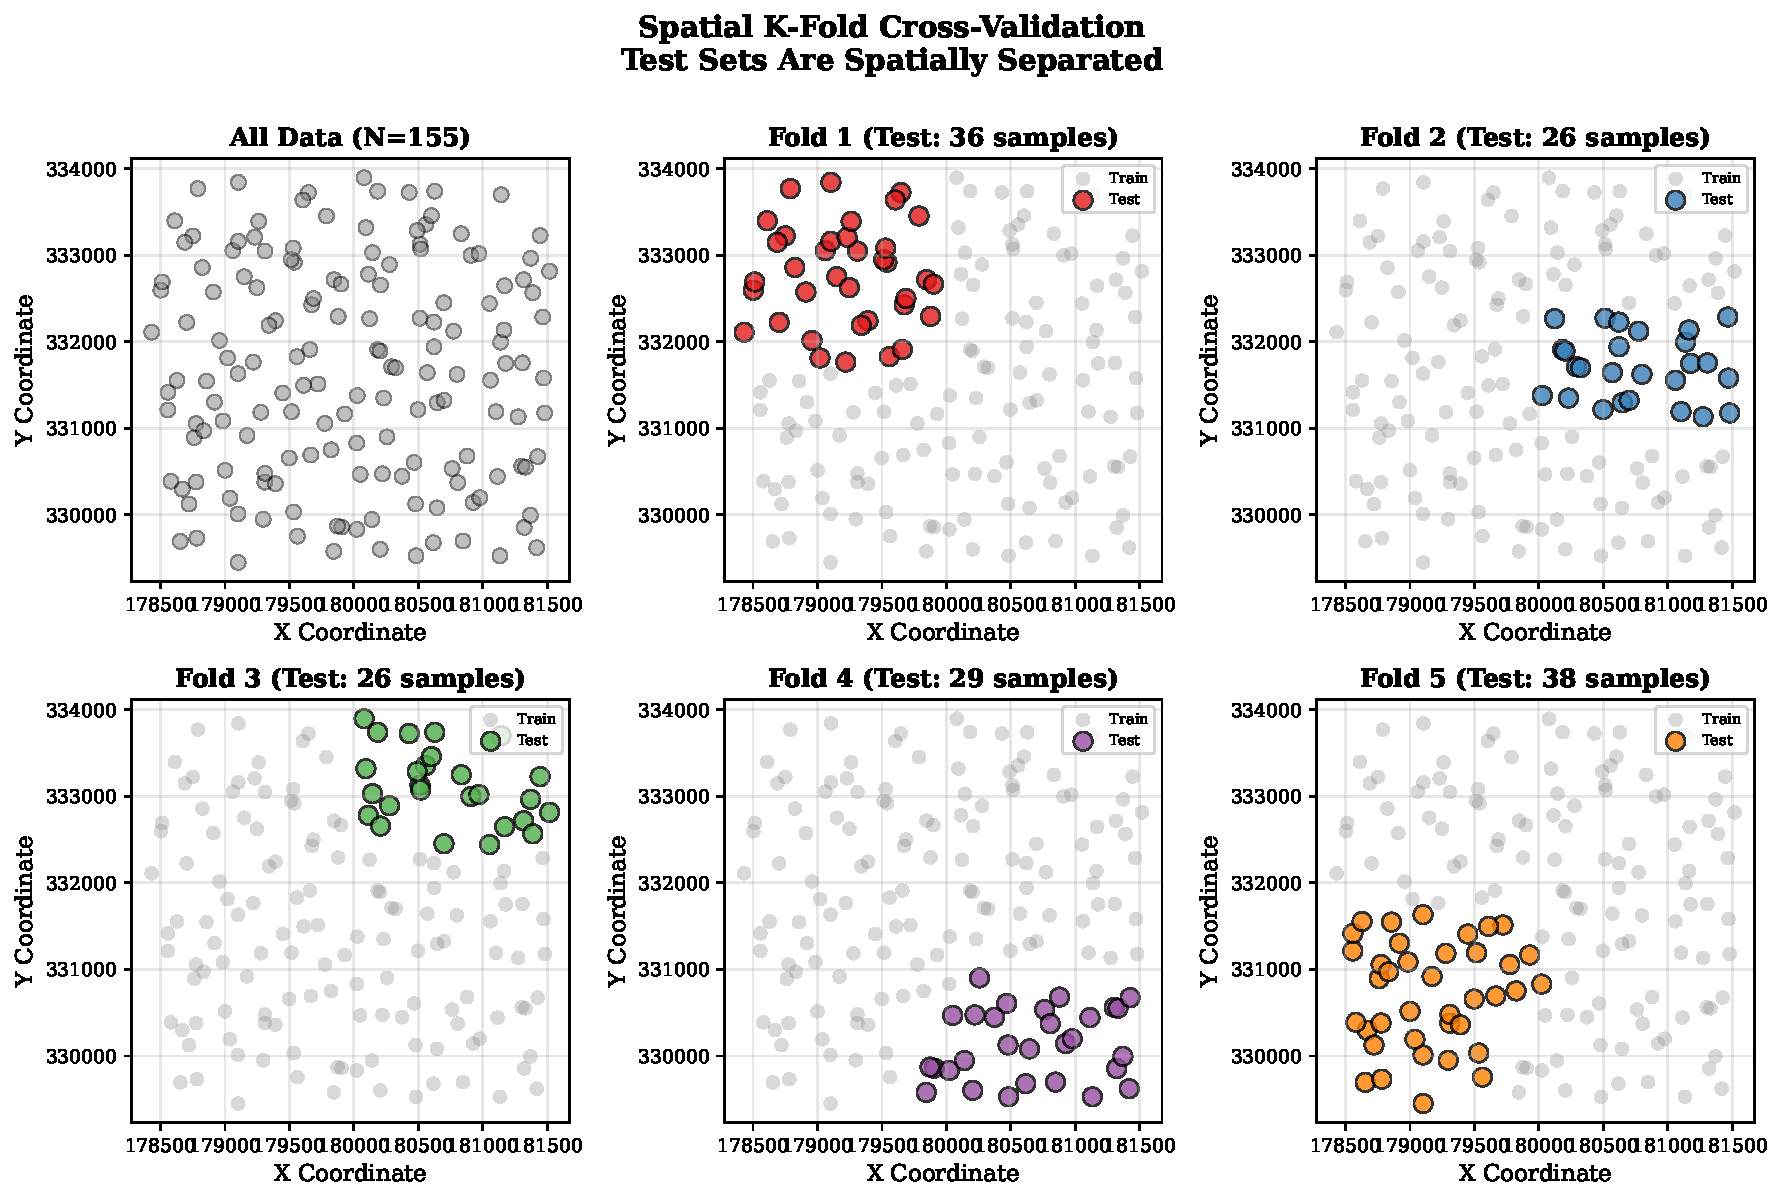
\includegraphics[width=0.95\textwidth]{figures/figure4_spatial_folds.pdf}
\caption{Spatial K-Fold cross-validation strategy. Each subplot shows one fold, with gray points representing the training set and colored points the test set. Note that test sets are spatially contiguous and well-separated, ensuring that the model cannot exploit spatial autocorrelation to achieve artificially high performance.}
\label{fig:spatial_folds}
\end{figure}

Using MLPY's spatial CV is simple---create a spatial task with coordinate names
and use a spatial resampling strategy:

\begin{lstlisting}[language=Python, caption=Spatial cross-validation in MLPY]
from mlpy.tasks import TaskRegrSpatial
from mlpy.resamplings.spatial import SpatialKFold
from mlpy.learners.sklearn import LearnerRandomForestRegressor
from mlpy.measures import MeasureRegrRMSE
from mlpy import resample

# Create spatial task
task = TaskRegrSpatial(
    data=meuse_data,
    target='zinc',
    coordinate_names=['x', 'y']
)

# Use spatial cross-validation
result = resample(
    task=task,
    learner=LearnerRandomForestRegressor(n_estimators=100),
    resampling=SpatialKFold(n_folds=5),
    measures=[MeasureRegrRMSE()]
)

# Get realistic error estimate
spatial_rmse = result.score('regr.rmse', average='mean')
# RMSE: 125.4 ppm (realistic estimate)

# Compare with regular CV (for demonstration)
from mlpy.tasks import TaskRegr
from mlpy.resamplings import ResamplingCV

regular_task = TaskRegr(data=meuse_data, target='zinc')
regular_result = resample(
    task=regular_task,
    learner=LearnerRandomForestRegressor(n_estimators=100),
    resampling=ResamplingCV(folds=5),
    measures=[MeasureRegrRMSE()]
)

regular_rmse = regular_result.score('regr.rmse', average='mean')
# RMSE: 101.6 ppm (overly optimistic!)
\end{lstlisting}

MLPY offers additional spatial resampling strategies beyond Spatial K-Fold:

\begin{itemize}
\item \textbf{SpatialBlockCV}: Divides the spatial extent into a regular grid of blocks
\item \textbf{SpatialBufferCV}: Creates buffer zones around test sets to exclude nearby training data
\item \textbf{SpatialClusterCV}: Uses hierarchical clustering for spatial separation
\end{itemize}

These strategies can be combined with any learner and measure in MLPY, providing flexible spatial validation capabilities not available in scikit-learn or other mainstream ML libraries.

\subsubsection{Discussion and Implications}

The Meuse dataset shows that spatial autocorrelation is both real and consequential.
With Moran's I around 0.27, the spatial structure is strong enough to violate
CV's independence assumption. And the impact is substantial: regular CV
underestimates error by 19\%. This isn't a minor statistical curiosity---it
means a model that appears highly accurate will perform much worse when deployed
to new regions. Model selection would favor overfit models. Decisions based on
these inflated estimates could waste resources.

Sklearn and most Python ML frameworks don't handle this. MLPY does, with
spatial resampling strategies that integrate cleanly with the rest of the
framework.

\textbf{When to use spatial CV:} Use spatial cross-validation when data has
geographic coordinates, when you need to predict on new spatial regions, or
in domains like environmental science, ecology, epidemiology, and agriculture
where spatial structure is common.

\textbf{Related work:} Spatial validation is increasingly recognized as
critical~\citep{roberts2017cross, meyer2018improving, ploton2020spatial}.
R users have \texttt{blockCV}~\citep{valavi2019blockcv}. Python had nothing
comparable until MLPY.

This case study shows why MLPY exists: standard ML frameworks work fine for
textbook problems but fail on real-world data with structure. MLPY handles
spatial data, temporal data, and other cases where sklearn's assumptions break.
